\vsssub
\subsubsection{~$S_{uo}$：未解析障碍物源项} \label{sec:UOST}
\vsssub

\opthead{UOST}{\ws}{L. Mentaschi}

未解析的水深和海岸特征，例如海崖、浅滩和小岛，是谱波浪模型局地误差的重要来源。
它们的耗散效应会在长距离上传递和累积，忽略这些效应会损害大范围模型区域的模拟技巧
\citep{tol:Waves01a,tol:WaF02,art:Tuomi2014,art:Mentaschi2015a}。
在 \ws\ 中，对未解析障碍物造成的耗散进行次尺度建模有两种方法：
a) 一种已在规则网格上建立的基于传播的方法，见第 \ref{sub:num_obst} 节
\citep{tol:OMOD03a, tol:OMOD08a}；b) 本节描述的未解析障碍物源项
\citep[UOST,][]{art:Mentaschi2018a,art:Mentaschi2015b}。
除了几乎支持任意网格类型外，UOST 还考虑未解析特征的方向/空间布局；相对于既有方法，
这能提高模型技巧 \citep{art:HMM00,art:Mentaschi2018b}。

UOST 基于如下假设：任意网格都可视为一组称为单元的多边形，模型估计每个单元中未知量的
平均值。给定一个单元（称其为 A，图 \ref{fig:UOST}ab），UOST 对每个谱分量估计：
a) 位于 A 中的未解析特征的影响（局地耗散，LD）；b) 位于 A 上游并将其阴影投射到 A
上的未解析特征的影响（阴影效应，SE）。为估计 SE，对每个单元/谱分量定义一个上游多边形
A\textsc{\char13}，它是 A 的相邻联合单元（图 \ref{fig:UOST}ab 中的 B、C 和 D 单元）
与 A 上游通量的交集。对每个单元或上游多边形，以及每个谱分量，都估计两个不同的
透明度系数。1) 总体透明度系数 $\alpha$；2) 依赖布局的透明度 $\beta$，定义为从单元
上游侧开始的单元截面平均透明度。

源项可表示为

\begin{equation}
S_{uo} = S_{ld} + S_{se}\ ,
\end{equation}

\begin{equation}
S_{ld} = - \psi_{ld}(\mathbf{k}) \frac{1 - \beta_l(\mathbf{k})}{\beta_l(\mathbf{k})} \frac{c_g(\mathbf{k})}{\Delta L} N \ ,
\end{equation}

\begin{equation}
S_{se} = - \psi_{se}(\mathbf{k}) \bigg[ \frac{\beta_u(\mathbf{k})}{\alpha_u(\mathbf{k})} - 1 \bigg] \frac{c_g(\mathbf{k})}{\Delta L} N \ ,
\end{equation}

其中 $S_{ld}$ 和 $S_{se}$ 分别为局地耗散和阴影效应，$N$ 为谱密度，
$\mathbf{k}$ 为波矢，$c_g$ 为群速，$\Delta L$ 为谱分量在单元中的路径长度，
$\psi$ 因子表示存在局地波浪增长时耗散的减弱。$\alpha$ 和 $\beta$ 的下标 l 与 u
分别表示这些系数可对应于单元和上游多边形。关于 UOST 理论框架的更详细说明，请读者
参阅 \citep{art:Mentaschi2015b, art:Mentaschi2018a}。

\begin{figure} \begin{center}
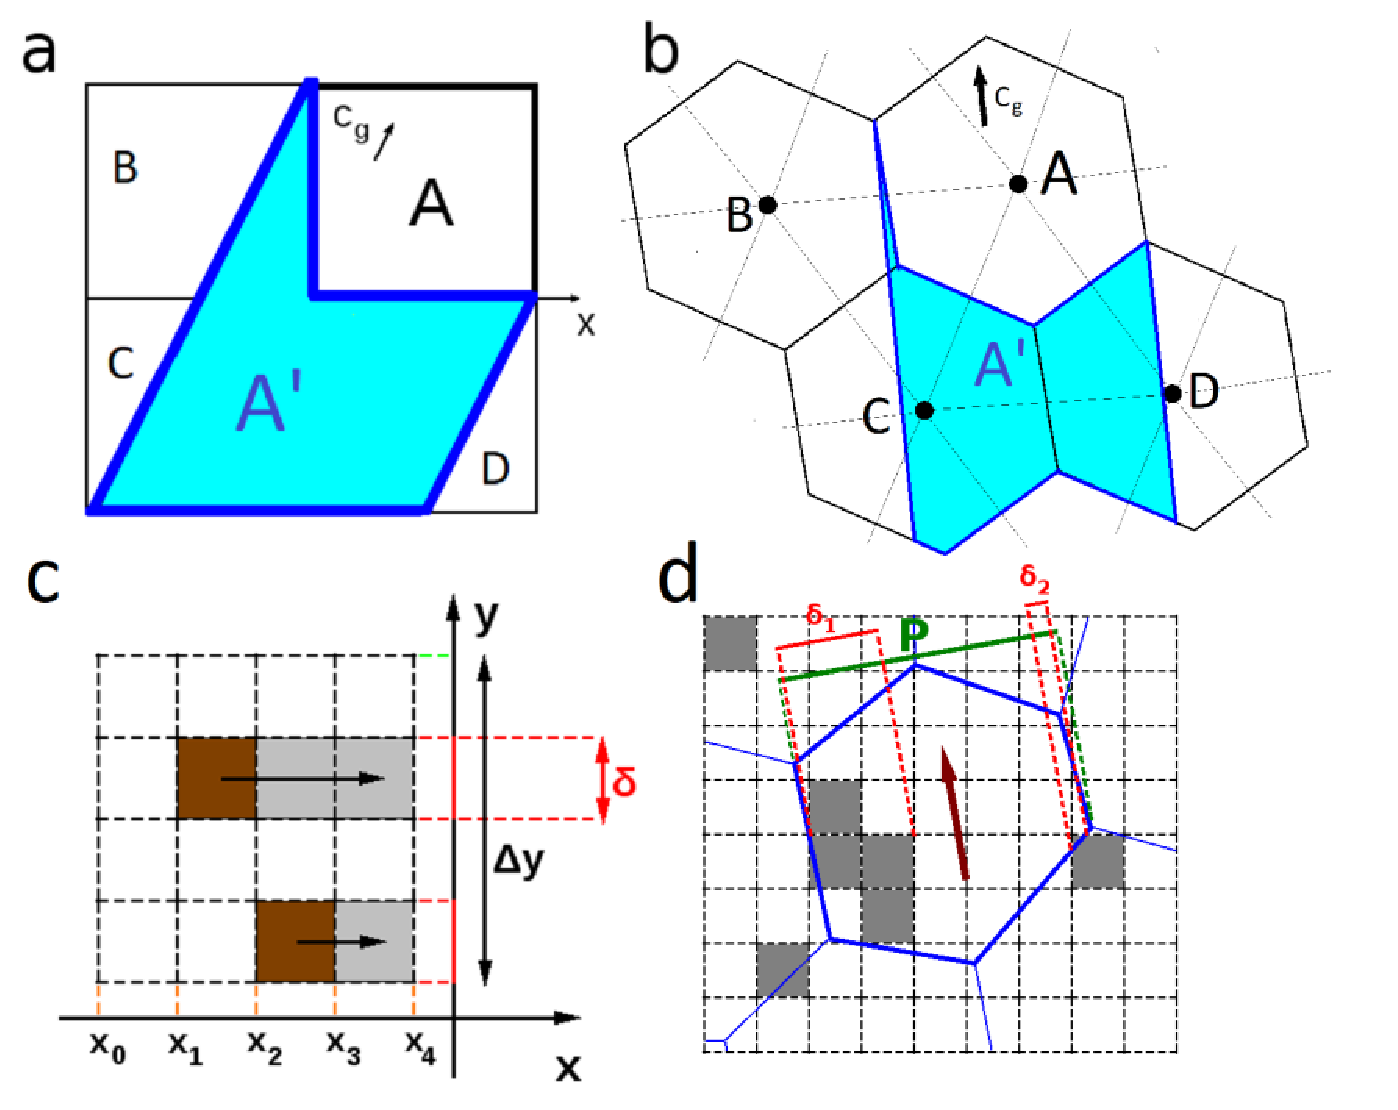
\epsfig{file=./eqs/UOST.eps,angle=0,width=4in}
\caption{
a：一个方形单元（A）及其上游多边形
（A\textsc{\char13}，由蓝线限定，以浅蓝色表示），对应以群速 $c_g$ 传播的谱分量。
联合 BCD 多边形表示邻域多边形。
b：同 a，但对应三角网格（六边形近似表示中值对偶单元）。
c：方形单元中 $\alpha$ 和 $\beta$ 的计算，$N_s=4$，谱分量沿 x 轴传播。
d：同 c，但对应六边形单元和倾斜谱分量。d 图中的灰色方块表示未解析障碍物。
}
\label{fig:UOST} \botline
\end{center}
\end{figure}

\textbf{网格参数的自动生成。}
开源 python 包 alphaBetaLab（https://github.com/menta78/alphaBetaLab）已被开发，
用于从真实世界水深自动估计上游多边形、透明度系数
$\alpha_l$、$\beta_l$、$\alpha_u$、$\beta_u$，以及 UOST 所需的其他参数。
alphaBetaLab 将单元视为自由多边形，并根据未解析障碍物相对于入射谱分量的横截面估计
透明度系数（图 \ref{fig:UOST}cd）。这意味着它可应用于任意类型网格，包括非结构三角
网格和 SMC 网格（截至 2018 年 8 月，仅处理规则网格和三角网格，但很快会加入对
SMC 网格的支持）。需要指出的是，虽然 UOST 本身能够使能量耗散随谱频率变化，但
alphaBetaLab 目前只考虑方向。关于 alphaBetaLab 中实现算法的更多细节，请用户参阅
\cite{art:Mentaschi2018a}。\cite{art:Mentaschi2018c} 提供了该软件及其架构的文档，
并给出了使用指导和示例。

\textbf{时间步设置。}
在 \ws\ 中，源项在每个全局时间步结束时施加。因此，为了在给定单元上正常工作，
UOST 要求全局时间步小于或等于该单元的临界 CFL 时间步，也就是最快谱分量完全穿过该
单元所需的时间。否则，部分能量会在未被阻挡的情况下穿过该单元 \citep{art:Mentaschi2018a}。

在单元大小差异很大的非结构网格中，如果把 UOST 应用于所有单元，包括最小单元，可能会
要求极小的全局时间步，从而影响模型经济性。为避免这一问题，用户可设置 alphaBetaLab
以忽略小于用户定义阈值的单元，然后在 \ws\ 中设置与该阈值相关的临界 CFL 时间步作为
全局时间步 \citep{art:Mentaschi2018c}。

\begin{table} \begin{center}
 \footnotesize
\begin{tabular}{|p{4cm}|p{2.5cm}|p{5.5cm}|} \hline \hline
Namelist 参数    &  说明           & 默认值 \\
\hline
  UOSTFILELOCAL &  局地 $\alpha$/$\beta$ 输入文件路径   &  obstructions\_local.\textit{gridname}.in    \\ \hline
  UOSTFILESHADOW &  阴影 $\alpha$/$\beta$ 输入文件路径   & obstructions\_shadow.\textit{gridname}.in   \\ \hline
  UOSTFACTORLOCAL &  局地透明度率定因子  &  1   \\ \hline
  UOSTFACTORSHADOW &  阴影透明度率定因子  &  1  \\
\hline
\end{tabular} \end{center}
\caption{UOST 参数、说明及默认值。} \label{tab:UOST}
\botline
\end{table}
